\documentclass[border=3pt,tikz, convert]{standalone}
\usepackage{amsmath} % for aligned
\usepackage{listofitems} % for \readlist to create arrays
\usetikzlibrary{arrows.meta} % for arrow size
\usepackage[outline]{contour} % glow around text
\contourlength{1.4pt}

% COLORS
\usepackage{xcolor}
\colorlet{myred}{red!80!black}
\colorlet{myblue}{blue!80!black}
\colorlet{mygreen}{green!60!black}
\colorlet{myorange}{orange!70!red!60!black}
\colorlet{mydarkred}{red!30!black}
\colorlet{mydarkblue}{blue!40!black}
\colorlet{mydarkgreen}{green!30!black}

% STYLES
\tikzset{
  >=latex, % for default LaTeX arrow head
  node/.style={thick,circle,draw=myblue,minimum size=22,inner sep=0.5,outer sep=0.6},
  node in/.style={node,green!20!black,draw=mygreen!30!black,fill=mygreen!25},
  node hidden/.style={node,blue!20!black,draw=myblue!30!black,fill=myblue!20},
  node convol/.style={node,orange!20!black,draw=myorange!30!black,fill=myorange!20},
  node out/.style={node,red!20!black,draw=myred!30!black,fill=myred!20},
  connect/.style={thick,mydarkblue}, %,line cap=round
  connect arrow/.style={-{Latex[length=4,width=3.5]},thick,mydarkblue,shorten <=0.5,shorten >=1},
  node 1/.style={node in}, % node styles, numbered for easy mapping with \nstyle
  node 2/.style={node hidden},
  node 3/.style={node out}
}
\def\nstyle{int(\lay<\Nnodlen?min(2,\lay):3)} % map layer number onto 1, 2, or 3

\begin{document}

% One hidden layer

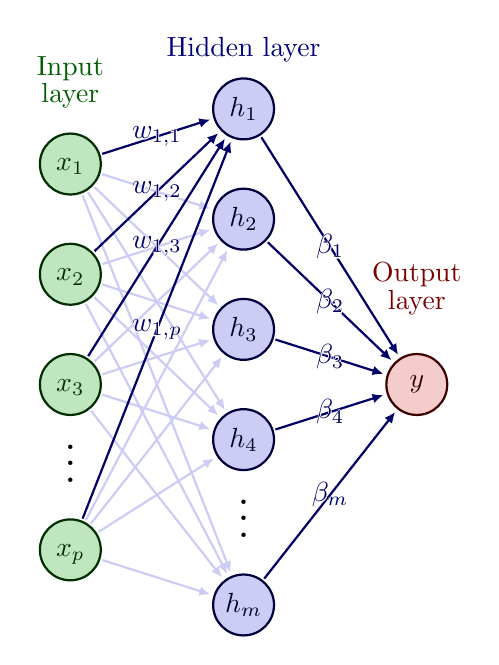
\begin{tikzpicture}[x=2.2cm,y=1.4cm]

    \readlist\Nnod{4,5,1} % array of number of nodes per layer
    \readlist\Nstr{p,m,1} % array of string number of nodes per layer
    \readlist\Cstr{\strut x,h,y} % array of coefficient symbol per layer
    \def\yshift{0.5} % shift last node for dots
    
    
    \foreachitem \N \in \Nnod{ % loop over layers
      \def\lay{\Ncnt} % alias of index of current layer
      \pgfmathsetmacro\prev{int(\Ncnt-1)} % number of prev layer
      
      % Nodes
      \foreach \i [evaluate={\c=int(\i==\N); \y=\N/2-\i-\c*\yshift;
                   \index=(\i<\N?int(\i):"\Nstr[\lay]");
                   \x=\lay; \n=\nstyle;}] in {1,...,\N}{ % loop over nodes
        
        \ifnum\N>1
          \node[node \n] (N\lay-\i) at (\x,\y) {$\Cstr[\lay]_{\index}$};
        \else
          \node[node \n] (N\lay-\i) at (\x,\y) {$\Cstr[\lay]$};
        \fi
      }
      
      % Dots between Nodes
      \ifnum\N>1
      	\path (N\lay-\N) --++ (0,1+\yshift) node[midway,scale=1.5] {$\vdots$};
      \fi
      
      % Connections
      \ifnum\lay=2 % connect to prev layer
        \foreach \j [evaluate={\index=(\j<\Nnod[\prev]?int(\j):"\Nstr[\prev]");}]in {1,...,\Nnod[\prev]}{ % loop over nodes in previous layer
          \foreach \i in {1,...,\N}{ 
          \ifnum\i=1
            \draw[connect arrow] (N\prev-\j) -- (N\lay-\i) 
              node[pos=0.50] {\contour{white}{$w_{1,\index}$}};
          \else
            \draw[connect arrow, myblue!20] (N\prev-\j) -- (N\lay-\i);
          \fi
          }
        }
      \fi
      
      \ifnum\lay=3 % connect to prev layer
      \foreach \j [evaluate={\index=(\j<\Nnod[\prev]?int(\j):"\Nstr[\prev]");}]in {1,...,\Nnod[\prev]}{ % loop over nodes in previous layer
          \draw[connect arrow] (N\prev-\j) -- (N\lay-1) 
            node[pos=0.50] {\contour{white}{$\beta_{\index}$}};
      }
    \fi 
    }
    
    % LABELS
    \node[above=5,align=center,mygreen!60!black] at (N1-1.90) {Input\\[-0.2em]layer};
    \node[above=2,align=center,myblue!60!black] at (N2-1.90) {Hidden layer};
    \node[above=10,align=center,myred!60!black] at (N\Nnodlen-1.90) {Output\\[-0.2em]layer};
    
  \end{tikzpicture}

% Multiple hidden layers

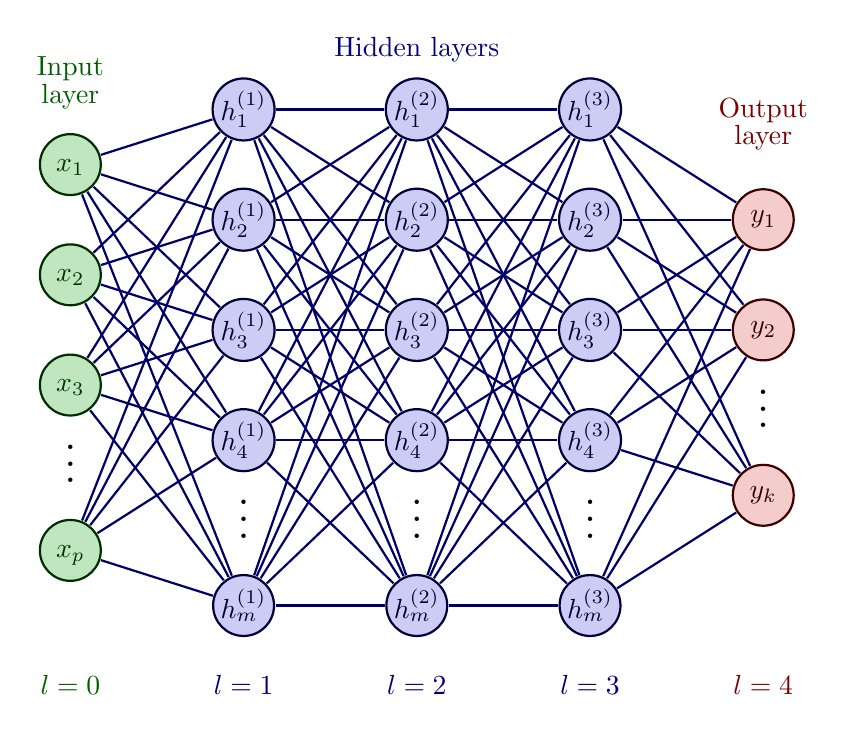
\begin{tikzpicture}[x=2.2cm,y=1.4cm]
    \message{^^JNeural network, shifted}
    \readlist\Nnod{4,5,5,5,3} % array of number of nodes per layer
    \readlist\Nstr{p,m,m,m,k} % array of string number of nodes per layer
    \readlist\Cstr{\strut x,h^{(\prev)},h^{(\prev)},h^{(\prev)},y} % array of coefficient symbol per layer
    \def\yshift{0.5} % shift last node for dots
    
    \message{^^J  Layer}
    \foreachitem \N \in \Nnod{ % loop over layers
      \def\lay{\Ncnt} % alias of index of current layer
      \pgfmathsetmacro\prev{int(\Ncnt-1)} % number of previous layer
      \message{\lay,}
      \foreach \i [evaluate={\c=int(\i==\N); \y=\N/2-\i-\c*\yshift;
                   \index=(\i<\N?int(\i):"\Nstr[\lay]");
                   \x=\lay; \n=\nstyle;}] in {1,...,\N}{ % loop over nodes
        % NODES
        \node[node \n] (N\lay-\i) at (\x,\y) {$\Cstr[\lay]_{\index}$};
        
        % CONNECTIONS
        \ifnum\lay>1 % connect to previous layer
          \foreach \j in {1,...,\Nnod[\prev]}{ % loop over nodes in previous layer
            \draw[connect] (N\prev-\j) -- (N\lay-\i);
          }
        \fi % else: nothing to connect first layer
        
      }
      \path (N\lay-\N) --++ (0,1+\yshift) node[midway,scale=1.5] {$\vdots$};
    }
    
    % LABELS
    \node[above=5,align=center,mygreen!60!black] at (N1-1.90) {Input\\[-0.2em]layer};
    \node[above=2,align=center,myblue!60!black] at (N3-1.90) {Hidden layers};
    \node[above=10,align=center,myred!60!black] at (N\Nnodlen-1.90) {Output\\[-0.2em]layer};

    \node[below=30,align=center,mygreen!60!black] at (N1-4.270) {$l=0$};
    \node[below=10,align=center,myblue!60!black] at (N2-5.270) {$l = 1$};
    \node[below=10,align=center,myblue!60!black] at (N3-5.270) {$l = 2$};
    \node[below=10,align=center,myblue!60!black] at (N4-5.270) {$l = 3$};
    \node[below=50,align=center,myred!60!black] at (N\Nnodlen-3.270) {$l=4$};
  \end{tikzpicture}



\end{document}